\documentclass[preprint,12pt]{elsarticle}

\input{math_commands.tex}

\usepackage[utf8]{inputenc}
\usepackage{amsmath}
\usepackage{amssymb}
\usepackage{booktabs}
\usepackage{graphicx}
\usepackage{hyperref}
\usepackage{url}
\usepackage{tikz}
\usetikzlibrary{shadows, arrows.meta, positioning, fit, backgrounds, shapes.geometric, arrows}

\begin{document}

\begin{frontmatter}

\title{Attention-Free Spiking Neural Networks for Efficient Sequence Representation}

% Author details removed for double-blind review

\begin{abstract}
Spiking Neural Networks (SNNs) provide an energy-efficient alternative to conventional Deep Neural Networks by utilizing discrete, event-driven temporal spikes. However, adopting Transformer-based paradigms into the spiking domain typically requires mapping complex Self-Attention mechanisms into spike operations. In this paper, we present an in-depth mathematical formulation and empirical ablation of a Spike-Driven Self-Attention layer—modeled around a Spike-Overlap-like spike intersection metric—to evaluate its true utility. Through comprehensive knowledge distillation, we demonstrate that incorporating Spike-Overlap Attention yields a severe execution bottleneck, quadrupling training time and doubling inference latency (with $\sim 3\times$ more parameters), while offering a negligible absolute accuracy gain (+0.0048 Pearson correlation). We propose a purely recurrent, attention-free Spiking Sentence Embedder operating exclusively through Leaky Integrate-and-Fire (LIF) pooling and Backpropagation Through Time (BPTT), incorporating an SNN-native hyperpolarization mechanism for sequence padding. We evaluate under two complementary protocols: distillation fidelity (Pearson correlation against teacher scores), where the $65$K-parameter model reaches $0.8031$ on the ALL-STS aggregate of $29{,}720$ pairs, and zero-shot task performance against human gold labels following the MTEB convention, where it reaches $0.7651$ Pearson / $0.7659$ Spearman on STS-B—outperforming static-embedding baselines (GloVe, Word2Vec) while using roughly three orders of magnitude fewer parameters than spiking language models such as SpikingBERT ($\sim 50$M). Replacing complex spatial attention routing with pure recurrent temporal pooling drastically reduces computational overhead, suggesting that spatial routing via self-attention provides marginal benefit relative to its cost for neuromorphic sequence representation tasks.
\end{abstract}

\end{frontmatter}

\section{Introduction}

The computational overhead of Dense Sentence Embedders \citep{devlin2018bert}, such as SBERT \citep{reimers2019sentence}, is heavily dominated by the dense matrix multiplications required in the standard Scaled Dot-Product Attention introduced by Vaswani et al. \cite{vaswani2017attention}. While numerous efficient Transformer architectures have been proposed to mitigate this quadratic $\mathcal{O}(L^2)$ complexity \citep{tay2022efficient}, they still rely fundamentally on continuous floating-point operations. Spiking Neural Networks (SNNs) alleviate this constraint by operating on sparse, event-driven additions rather than complex multiplications, making them highly suitable for highly parallel neuromorphic hardware \citep{roy2019towards}. Recent neuromorphic NLP research has focused on translating Self-Attention to SNNs \citep{li2022spikeformer, zhu2023spikegpt} and extending these architectures to extract semantic embeddings. Specific attention mechanisms, such as the Sparse Coincidence-Based Semantic Attention \citep{coincidence2026}, rely heavily on spike overlaps. Furthermore, the development of specialized frameworks like SpikingJelly \citep{fang2023spikingjelly} has accelerated the validation of surrogate gradient methods in deep architectures. However, a critical bottleneck persists: forcibly mapping continuous $\mathcal{O}(L^2)$ spatial attention mechanisms into the discrete spiking domain drastically inflates computational overhead, largely negating the inherent efficiency of SNNs. This raises a fundamental architectural question: \textit{Are explicit spatial attention mechanisms truly necessary for sequence representation, or can the native temporal recurrence of SNNs suffice?}

In this study, we systematically deconstruct the forward dynamics and learning mechanisms of an SNN sequence embedder. We mathematically formulate a Spike-Overlap-based Attention algorithm and utilize it as a comparative baseline to expose the computational inefficiencies of spatial routing. We contrast this against our proposed attention-free Recurrent Pooler. Our empirical findings provide strong evidence that forcing spatial attention onto SNNs is computationally unjustifiable for this task. Instead, the native temporal integration capabilities of the recurrent pooler, when optimized via Backpropagation Through Time (BPTT) and Surrogate Gradients, are overwhelmingly sufficient for encoding complex semantic structures.

\subsection*{Contributions}
Our primary contribution in this study is the proposal and rigorous evaluation of an \textbf{Attention-Free Recurrent Spiking Sentence Embedder}. By bypassing complex $\mathcal{O}(L^2)$ spatial routing mechanisms and relying exclusively on temporal Leaky Integrate-and-Fire (LIF) pooling optimized via Backpropagation Through Time (BPTT), we demonstrate that temporal integration is overwhelmingly sufficient for semantic encoding. This minimalist architecture achieves comparable semantic fidelity to spatial attention baselines while offering a $4\times$ reduction in training cost and a $2\times$ reduction in inference latency. 

To support and evaluate this primary architecture, we implemented several supporting methodologies:
\begin{itemize}
    \item A mathematical formulation of Spike-Driven Spike-Overlap Attention, which serves purely as a comparative baseline to expose the computational bottlenecks of spatial routing in SNNs.
    \item \textbf{Hyperpolarized Padding}, an SNN-native sequence padding mechanism that forces padding tokens into a negative refractory state to prevent noise accumulation.
    \item \textbf{Add-Only Delta BPTT routing}, a gradient routing technique that simplifies computations and significantly reduces floating-point matrix multiplications during the backward pass.
    \item A \textbf{dual-protocol evaluation}—distillation fidelity against teacher scores and zero-shot task performance against human gold labels—situating the model against published SNN language models, efficient Transformers, and static-embedding baselines, with energy claims stated explicitly as operation-count proxies under a standard 45\,nm model.
\end{itemize}

\section{Related Work}

\subsection{Spiking Neural Networks for Language}
Recent work has begun porting Transformer primitives into the spiking domain. SpikFormer \citep{zhou2023spikformer} introduced spike-driven self-attention for vision tasks, and SpikeGPT \citep{zhu2023spikegpt} scaled spiking architectures to generative language modeling with up to 216M parameters. For encoder-style representations, SpikeBERT \citep{lv2023spikebert} applies two-stage knowledge distillation from BERT, while SpikingBERT \citep{bal2024spikingbert} integrates spiking neurons with BERT-style pretraining and reports GLUE results—including a Spearman correlation of $0.819$ on STS-B—with approximately $50$M parameters; Spikingformer \citep{zhou2025spikingformer} stabilizes spike-driven residual learning and reports $0.545$ on STS-B with $66$M parameters. Two observations motivate our study. First, all of these models retain an explicit $\mathcal{O}(L^2)$ attention mechanism, which dominates their operation counts. Second, none of them target \emph{sentence embeddings} or evaluate on the standard STS suite (STS-12 through STS-16, STS-B, SICK-R) against human judgments; to our knowledge, our $65$K-parameter recurrent embedder is the first SNN evaluated directly on this suite.

\subsection{Efficient Sentence Embedding}
Dense sentence embedders are typically obtained by fine-tuning pretrained encoders with siamese objectives \citep{reimers2019sentence} or contrastive objectives \citep{gao2021simcse}, and compressed via knowledge distillation \citep{hinton2015distilling, sanh2019distilbert, wang2020minilm} or post-hoc quantization. These models define the accuracy frontier—DistilBERT reports $0.869$ Spearman on STS-B \citep{sanh2019distilbert}—but rely fundamentally on continuous floating-point matrix multiplications. Static embeddings with mean pooling (Word2Vec, GloVe) remain competitive low-cost baselines and are included in our evaluation. The standard evaluation convention for this task family is Spearman rank correlation against human gold labels \citep{muennighoff2022mteb, cer2017semeval}, which we adopt for the task-performance track of our evaluation.

\subsection{Energy Accounting for SNNs}
SNN efficiency claims conventionally rely on operation counting: spike-driven accumulate operations (SOPs/ACs) are contrasted with multiply--accumulate operations (MACs), weighted by the 45\,nm energy figures of \citet{horowitz2014computing} ($0.9$\,pJ per 32-bit accumulation versus $4.6$\,pJ per 32-bit MAC) \citep{zhou2023spikformer, fang2023spikingjelly}. This proxy omits memory access and data movement, which can dominate real energy budgets. We therefore report both the theoretical proxy and measured CPU latency, and treat the proxy strictly as an upper bound.

\section{Methodology: Architectural Dynamics and BPTT}

\begin{figure}[t!]
\begin{center}
\resizebox{0.95\textwidth}{!}{%
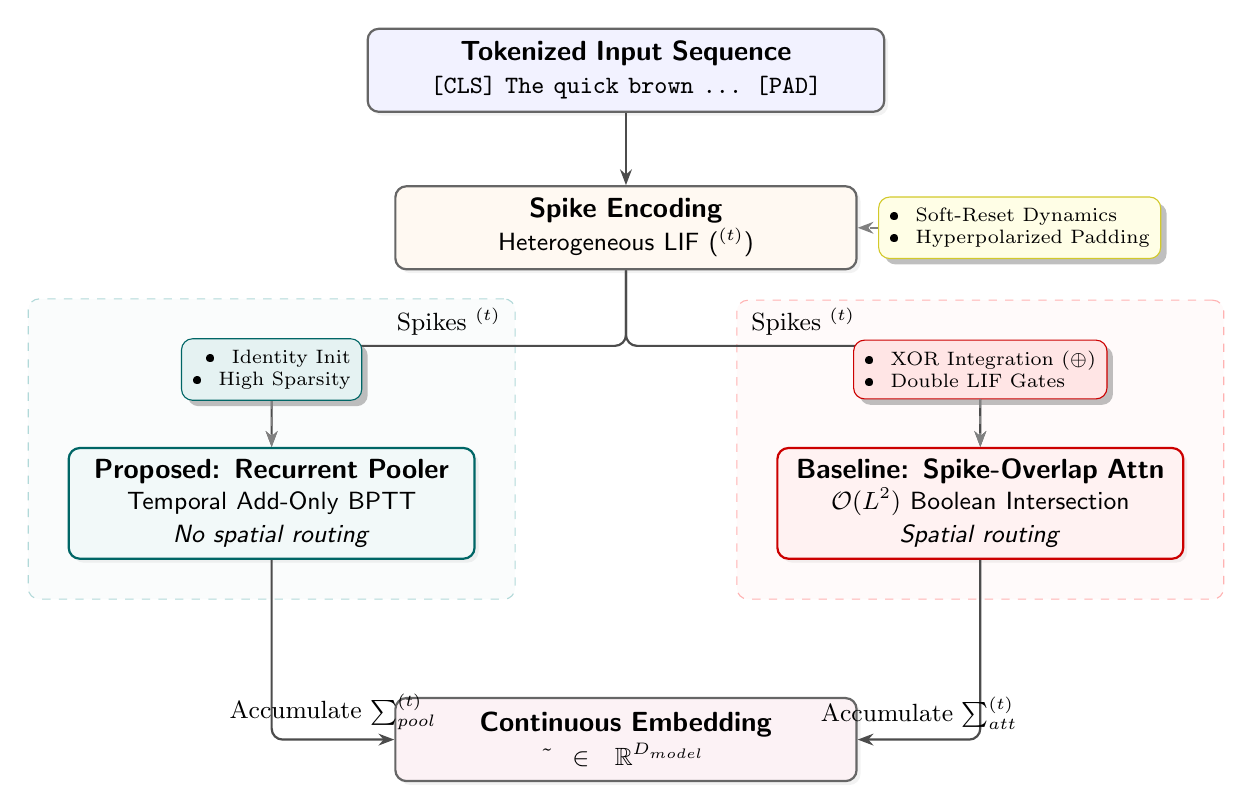
\begin{tikzpicture}[
    font=\sffamily,
    base/.style={rectangle, rounded corners, draw=black!60, thick, minimum height=3em, align=center, fill=white, drop shadow={opacity=0.1, shadow xshift=0.05cm, shadow yshift=-0.05cm}},
    input/.style={base, fill=blue!5, text width=18em},
    spike/.style={base, fill=orange!5, text width=16em},
    pooler/.style={base, fill=teal!5, text width=14em, minimum height=4em, draw=teal!80!black},
    attn/.style={base, fill=red!5, text width=14em, minimum height=4em, draw=red!80!black},
    output/.style={base, fill=purple!5, text width=16em},
    arrow/.style={-{Stealth[length=2mm]}, thick, draw=black!70},
    dashed_arrow/.style={-{Stealth[length=2mm]}, dashed, thick, draw=black!50}
]

% Center column
\node[input] (tokens) at (0, 0) {\textbf{Tokenized Input Sequence} \\ \small \texttt{[CLS] The quick brown ... [PAD]}};
\node[spike] (lif) at (0, -2) {\textbf{Spike Encoding} \\ \small Heterogeneous LIF ($\mV^{(t)}$)};
\draw[arrow] (tokens) -- (lif);

% Left branch (Proposed)
\node[pooler] (recurrent) at (-4.5, -5.5) {\textbf{Proposed: Recurrent Pooler} \\ \small Temporal Add-Only BPTT \\ \small \textit{No spatial routing}};

% Right branch (Baseline)
\node[attn] (attention) at (4.5, -5.5) {\textbf{Baseline: Spike-Overlap Attn} \\ \small $\mathcal{O}(L^2)$ Boolean Intersection \\ \small \textit{Spatial routing}};

% Split paths
\draw[arrow, rounded corners] (lif) -- (0, -3.5) -| node[above, pos=0.25, font=\small, text=black] {Spikes $\mS^{(t)}$} (recurrent);
\draw[arrow, rounded corners] (lif) -- (0, -3.5) -| node[above, pos=0.25, font=\small, text=black] {Spikes $\mS^{(t)}$} (attention);

% Output
\node[output] (out) at (0, -8.5) {\textbf{Continuous Embedding} \\ \small $\tilde{\mE} \in \mathbb{R}^{D_{model}}$};

% Join paths
\draw[arrow, rounded corners] (recurrent) |- node[above, pos=0.75, font=\small, text=black] {Accumulate $\sum \mV_{pool}^{(t)}$} (out);
\draw[arrow, rounded corners] (attention) |- node[above, pos=0.75, font=\small, text=black] {Accumulate $\sum \mV_{att}^{(t)}$} (out);

% Annotations
\node[align=left, font=\scriptsize, text=black, fill=yellow!10, draw=yellow!80!black, rounded corners, inner sep=4pt, drop shadow] (note1) at (5, -2) {\textbullet~ Soft-Reset Dynamics \\ \textbullet~ Hyperpolarized Padding};
\draw[dashed_arrow] (note1) -- (lif);

\node[align=right, font=\scriptsize, text=black, fill=teal!10, draw=teal!80!black, rounded corners, inner sep=4pt, drop shadow] (note2) at (-4.5, -3.8) {\textbullet~ Identity Init \\ \textbullet~ High Sparsity};
\draw[dashed_arrow] (note2) -- (recurrent);

\node[align=left, font=\scriptsize, text=black, fill=red!10, draw=red!80!black, rounded corners, inner sep=4pt, drop shadow] (note3) at (4.5, -3.8) {\textbullet~ XOR Integration ($\oplus$) \\ \textbullet~ Double LIF Gates};
\draw[dashed_arrow] (note3) -- (attention);

% Background groupings
\begin{scope}[on background layer]
    \node[fill=teal!2, rounded corners, draw=teal!30, dashed, inner sep=0.5cm, fit=(recurrent) (note2)] {};
    \node[fill=red!2, rounded corners, draw=red!30, dashed, inner sep=0.5cm, fit=(attention) (note3)] {};
\end{scope}

\end{tikzpicture}%
}
\end{center}
\caption{Architectural flowchart contrasting the proposed minimalist Recurrent Pooler against the $\mathcal{O}(L^2)$ Spike-Overlap Attention baseline. The Recurrent Pooler completely bypasses quadratic spatial routing, natively translating discrete token spikes into a continuous temporal embedding state.}
\label{fig:architecture}
\end{figure}

Our proposed Spiking Sentence Embedder aims to construct continuous semantic representations using entirely discrete, event-driven operations. The pipeline consists of Spike Encoding, a comparative Attention vs. Pooling mechanism, and Knowledge Distillation.

\subsection{Spike Encoding and Heterogeneous Dynamics}
Raw text is tokenized into vocabulary indices. The Spiking Embedding Layer translates these tokens into temporal spike trains $\mS_{emb}^{(t)}$ over discrete sequence steps $t \in [1, L]$, where the temporal dimension maps perfectly to sequence length. The membrane potential $\mV_{emb}^{(t)}$ is modeled via Leaky Integrate-and-Fire (LIF) dynamics:
\begin{equation}
\mV_{emb}^{(t)} = \min\left(1.0, \bm{\beta}_{emb} \odot \mV_{emb}^{(t-1)} + \mX^{(t)} \mW_{emb}\right) - \mS_{emb}^{(t)} \odot \bm{\theta}_{emb}
\end{equation}
When the pre-reset potential exceeds the threshold $\bm{\theta}_{emb}$, a spike $\mS_{emb}^{(t)} = 1$ is fired. We utilize a \textit{Soft-Reset} strategy (subtracting the threshold) rather than a hard reset to absolute zero. Preserving these fractional sub-threshold residual potentials prevents catastrophic semantic information loss across time. Furthermore, we introduce biological heterogeneity: the leak decay $\bm{\beta}_{emb}$ and thresholds $\bm{\theta}_{emb}$ are initialized with unique, uniformly distributed values across dimensions (e.g., $\beta \in [1 - 2^{-2}, 1 - 2^{-7}]$). This forces multi-timescale temporal processing immediately upon sequence ingestion. 

\textbf{Sequence Padding and Hyperpolarization:} To handle variable sequence lengths efficiently without relying on explicit attention padding masks, we introduce an SNN-native hyperpolarization technique. The embedding weights associated with the `<PAD>` token (index 0) are explicitly overridden to $-1.0$. Consequently, during padding time-steps, the incoming synaptic dot product yields a strongly negative current, hyperpolarizing the membrane potential ($V < 0$). This guarantees that padding tokens emit exactly zero spikes, completely eliminating noise accumulation during temporal pooling.

\subsection{Ablation Baseline: Spike-Driven Spike-Overlap Attention}
To evaluate the impact of spatial routing, we formalized a Spike-Driven Self-Attention mechanism as our ablation baseline. Unlike floating-point dot products, this method computes affinities purely through Boolean spike intersections (Spike-Overlap index numerator).
Embedding spikes $\mS_{emb}$ are projected into Query ($Q$), Key ($K$), and Value ($V$) spikes using independent LIF neurons. For any query token $i$ and key token $j$, the raw overlap is captured via a match count:
\begin{equation}
\mM_{i,j}^{(t)} = \sum_{d=1}^{D_{model}} \left( \mQ_{i,d}^{(t)} \wedge \mK_{j,d}^{(t)} \right)
\end{equation}
These integer match counts are normalized by the maximum active sequence matches $\max_k (M_{i,k}^{(t)} + \epsilon)$. To maintain the purely spiking pipeline, these normalized fractional scores are passed into an auxiliary set of LIF neurons to generate attention mask spikes $\mS_{scores}$, which finally gate the Value spikes $V$ via accumulation.
While this avoids continuous floating-point multiplications, calculating $\mathcal{O}(L^2 \cdot D_{model})$ Boolean intersections at every single time-step, followed by dual-layered LIF dynamics, imposes severe computational bottlenecks and dramatically inflates execution time.

\textbf{Spike-Difference (XOR) Integration:} Following the generation of the attention-gated spikes (denoted as $\mS_{att}^{(t)}$), we integrate these contextual features with the original embedding spikes $\mS_{emb}^{(t)}$ using an exclusive-OR (XOR) logical operation: 
\begin{equation}
\mS_{agg}^{(t)} = \mS_{emb}^{(t)} \oplus \mS_{att}^{(t)}
\end{equation}
Unlike traditional additive residual connections, this XOR integration acts as an ``innovation signal.'' It isolates the feature discrepancy between the local token representation and the global contextual attention. By neutralizing redundant spikes that are active in both the local embedding and global context, the subsequent recurrent pooler is forced to process strictly the novel semantic shifts introduced by the attention layer. This integration is explicitly applied in all our attention-based evaluations.

\begin{figure}[t!]
\begin{center}
\resizebox{0.85\textwidth}{!}{%
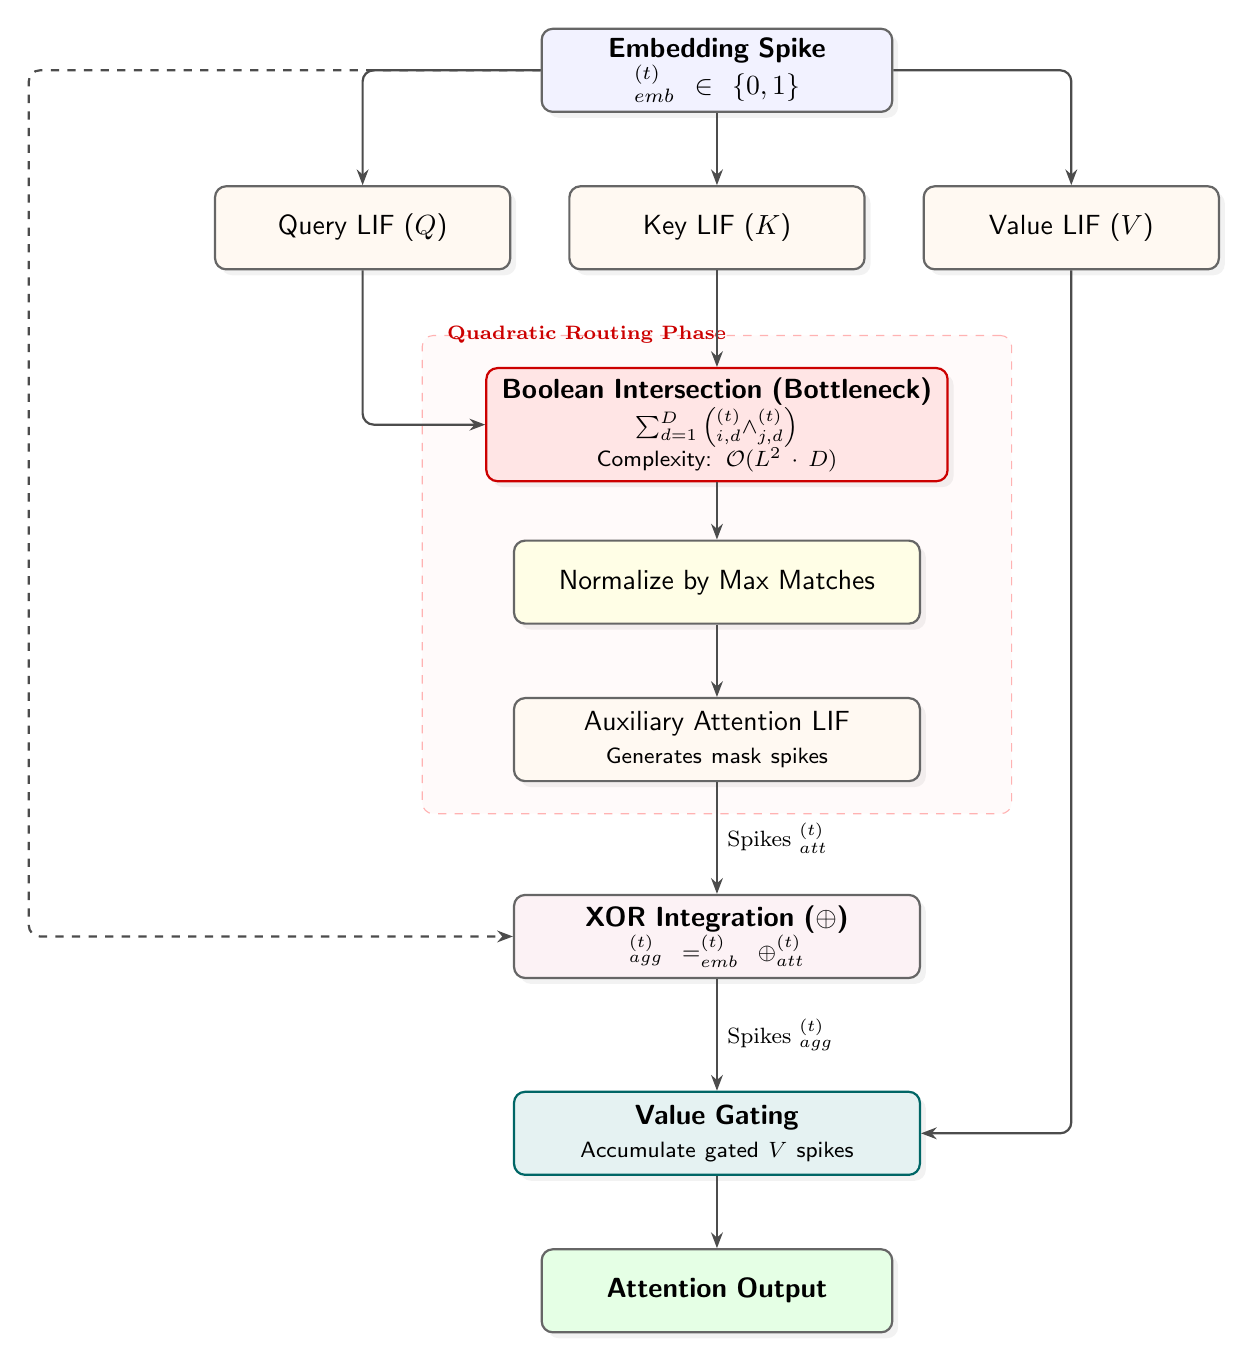
\begin{tikzpicture}[
    font=\sffamily,
    base/.style={rectangle, rounded corners, draw=black!60, thick, minimum height=3em, align=center, fill=white, drop shadow={opacity=0.1}},
    input/.style={base, fill=blue!5, text width=12em},
    proj/.style={base, fill=orange!5, text width=10em},
    compute/.style={base, fill=red!10, draw=red!80!black, text width=16em},
    gate/.style={base, fill=purple!5, text width=14em},
    arrow/.style={-{Stealth[length=2mm]}, thick, draw=black!70}
]

\node[input] (semb) at (0, 0) {\textbf{Embedding Spike} \\ $\mS_{emb}^{(t)} \in \{0,1\}$};
\node[proj] (k) at (0, -2) {Key LIF ($K$)};
\node[proj] (q) at (-4.5, -2) {Query LIF ($Q$)};
\node[proj] (v) at (4.5, -2) {Value LIF ($V$)};

\draw[arrow] (semb) -- (k);
\draw[arrow, rounded corners] (semb) -| (q);
\draw[arrow, rounded corners] (semb) -| (v);

\node[compute] (intersect) at (0, -4.5) {\textbf{Boolean Intersection (Bottleneck)} \\ \footnotesize $\sum_{d=1}^{D} \left( \mQ_{i,d}^{(t)} \wedge \mK_{j,d}^{(t)} \right)$ \\ \footnotesize Complexity: $\mathcal{O}(L^2 \cdot D)$};
\draw[arrow, rounded corners] (q) |- (intersect);
\draw[arrow] (k) -- (intersect);

\node[base, fill=yellow!10, text width=14em] (norm) at (0, -6.5) {Normalize by Max Matches};
\draw[arrow] (intersect) -- (norm);

\node[proj, text width=14em] (aux) at (0, -8.5) {Auxiliary Attention LIF \\ \footnotesize Generates mask spikes};
\draw[arrow] (norm) -- (aux);

\node[gate] (xor) at (0, -11) {\textbf{XOR Integration ($\oplus$)} \\ \footnotesize $\mS_{agg}^{(t)} = \mS_{emb}^{(t)} \oplus \mS_{att}^{(t)}$};
\draw[arrow] (aux) -- node[right, font=\footnotesize] {Spikes $\mS_{att}^{(t)}$} (xor);
\draw[arrow, rounded corners, dashed] (semb.west) -- ++(-6.5,0) |- (xor.west);

\node[gate, fill=teal!10, draw=teal!80!black] (gate_node) at (0, -13.5) {\textbf{Value Gating} \\ \footnotesize Accumulate gated $V$ spikes};
\draw[arrow] (xor) -- node[right, font=\footnotesize] {Spikes $\mS_{agg}^{(t)}$} (gate_node);
\draw[arrow, rounded corners] (v.south) |- (gate_node.east);

\node[input, fill=green!10] (out) at (0, -15.5) {\textbf{Attention Output}};
\draw[arrow] (gate_node) -- (out);

\begin{scope}[on background layer]
    \node[fill=red!2, rounded corners, draw=red!30, dashed, inner xsep=0.8cm, inner ysep=0.4cm, fit=(intersect) (norm) (aux)] (bg_attn) {};
    \node[right=0.2cm of bg_attn.north west, font=\scriptsize\bfseries, text=red!80!black] {Quadratic Routing Phase};
\end{scope}

\end{tikzpicture}%
}
\end{center}
\caption{Detailed computational flow of the Spike-Overlap Attention mechanism at a single timestep.}
\label{fig:attention_mech}
\end{figure}


\subsection{The Superior Recurrent Pooler (Proposed Architecture)}
We propose that spatial attention is functionally redundant. In our purely recurrent architecture, $\mS_{emb}^{(t)}$ bypasses attention and directly feeds into a Spiking Dense BPTT Pooler layer. Because the input spike $\mS_{emb}$ strictly guarantees binary values $\{0, 1\}$, the dense matrix projection is simplified to conditional accumulations:
\begin{equation}
\mX_{pool}^{(t)} = \sum_{d=1}^{D_{in}} \mW_{d} \cdot \mathbb{I}\left[ S_{emb, d}^{(t)} = 1 \right]
\end{equation}
By bypassing floating-point multiplications entirely, this step offers massive computational sparsity. The final continuous sentence embedding $E$ is extracted by accumulating the fractional membrane potentials across the entire temporal sequence $T$:
\begin{equation}
E = \sum_{t=1}^T \mV_{pool}^{(t)}
\end{equation}

\textbf{Learning via BPTT and Add-Only Deltas:} The true power of this architecture stems from its backpropagation mechanics. Because the Heaviside step function lacks a valid derivative, we employ a Rectangular Surrogate Mask to propagate errors, building upon the foundations of spatio-temporal backpropagation in SNNs \citep{neftci2019surrogate}:
\begin{equation}
\sigma'\big(\mV^{(t)}\big) = \begin{cases} 1 & \text{if } \big|\mV^{(t)} - \theta\big| < w \\ 0 & \text{otherwise} \end{cases}
\end{equation}
where $w$ represents the surrogate window width, dictating the range around the threshold $\theta$ where gradients are allowed to pass. During Backpropagation Through Time, the error $\delta^{(t)}$ at sequence step $t$ is explicitly linked to future time steps via the heterogeneous decay $\bm{\beta}_{pool}$:
\begin{equation}
\tilde{\bm{\delta}}^{(t)} = \left( \bm{\delta}_{out}^{(t)} + \tilde{\bm{\delta}}^{(t+1)} \odot \bm{\beta}_{pool} \right) \odot \sigma'\big(\mV_{pool}^{(t)}\big)
\end{equation}
This explicit temporal unrolling allows the $\beta$ parameter to act as a natural contextual router. The pooler inherently learns long-term syntactic dependencies simply by preserving or decaying gradients. Furthermore, during weight updating, the gradient accumulation $\Delta \mW$ also utilizes an Add-Only Delta rule:
\begin{equation}
\Delta \mW_{in, out} = \sum_{t=1}^{T} \tilde{\bm{\delta}}^{(t)}_{out} \cdot \mathbb{I}\left[ S_{emb, in}^{(t)} = 1 \right]
\end{equation}
This greatly reduces dense matrix multiplications in the forward and BPTT routing phases, rendering the spatial $\mathcal{O}(L^2)$ matrix completely unnecessary. To perfectly preserve the sequence representation at initialization before learning temporal dynamics, the pooler is initialized as an Identity Matrix with biases disabled. We use a rectangular surrogate window width of $w=1.0$.

\begin{figure}[t!]
\begin{center}
\resizebox{0.75\textwidth}{!}{%
\begin{tikzpicture}[
    font=\sffamily,
    base/.style={rectangle, rounded corners, draw=black!60, thick, minimum height=3em, align=center, fill=white, drop shadow={opacity=0.1}},
    input/.style={base, fill=blue!5, text width=16em},
    decision/.style={diamond, aspect=2, draw=orange!80!black, fill=orange!10, thick, text width=6em, align=center, drop shadow={opacity=0.1}},
    action/.style={base, fill=teal!10, draw=teal!80!black, text width=12em},
    skip/.style={base, fill=gray!10, draw=gray!60, text width=12em, dashed},
    state/.style={base, fill=purple!5, text width=16em},
    arrow/.style={-{Stealth[length=2mm]}, thick, draw=black!70}
]

\node[input] (semb) at (0,0) {\textbf{Input Spike} \\ $\mS_{emb}^{(t)} \in \{0,1\}$};

\node[decision] (cond) at (0, -2.5) {$\mS_{emb}^{(t)} == 1$};
\draw[arrow] (semb) -- (cond);

\node[action] (add) at (-4, -5) {\textbf{Add-Only Operation} \\ $\mV_{pool} \gets \mV_{pool} + \mW_{d}$};
\node[skip] (skip_node) at (4, -5) {\textbf{Skip (Sparsity)} \\ \footnotesize No MAC operations};

\draw[arrow, rounded corners] (cond.west) -| node[above left, font=\small\bfseries, text=teal!80!black] {True (Spike)} (add.north);
\draw[arrow, rounded corners] (cond.east) -| node[above right, font=\small\bfseries, text=gray!80!black] {False (Silence)} (skip_node.north);

\node[state] (vpool) at (0, -8) {\textbf{Membrane Potential} \\ $\mV_{pool}^{(t)}$};
\draw[arrow, rounded corners] (add.south) |- (vpool.west);
\draw[arrow, rounded corners] (skip_node.south) |- (vpool.east);

\node[action, fill=yellow!10, draw=yellow!80!black] (decay) at (0, -10.5) {\textbf{Heterogeneous Decay} \\ $\mV_{pool}^{(t)} \gets \mV_{pool}^{(t)} \odot \bm{\beta}_{pool}$};
\draw[arrow] (vpool) -- (decay);

\node[state, fill=blue!10] (acc) at (0, -13) {\textbf{Sequence Accumulation} \\ $\mE = \sum_{t=1}^T \mV_{pool}^{(t)}$};
\draw[arrow] (decay) -- (acc);

\node[input, fill=green!10, text width=18em] (out) at (0, -15.5) {\textbf{Final Continuous Embedding} \\ $\tilde{\mE} \in \mathbb{R}^{D_{model}}$};
\draw[arrow] (acc) -- (out);

\begin{scope}[on background layer]
    \node[fill=teal!2, rounded corners, draw=teal!30, dashed, inner xsep=1cm, inner ysep=0.5cm, fit=(cond) (add) (skip_node) (vpool)] (bg_sparse) {};
    \node[right=0.2cm of bg_sparse.north west, font=\scriptsize\bfseries, text=teal!80!black] {Sparse Event-Driven Update};
\end{scope}

\end{tikzpicture}%
}
\end{center}
\caption{Internal computational flow of the purely recurrent Add-Only Pooler. Floating-point multiplications are completely eliminated.}
\label{fig:pooler_mech}
\end{figure}


\subsection{Knowledge Distillation and Error Routing}
To optimize these dynamics, we distill "dark knowledge" from a pre-trained dense Teacher, adapting established knowledge distillation techniques \citep{hinton2015distilling} to the discrete spiking domain. We utilize a Mean Squared Error (MSE) objective over the Pearson Correlation scores. The exact error $\mathcal{E}$ is given by:
\begin{equation}
\mathcal{E} = \text{Sim}_{Teacher} - \sum_{d=1}^{D_{model}} \left(\tilde{\mE}_{1,d} \cdot \tilde{\mE}_{2,d}\right)
\end{equation}
where $\tilde{\mE}$ denotes the L2 unit-norm normalized, mean-centered pooled embeddings. The error gradient is derived symmetrically across the representation space:
\begin{align}
\frac{\partial \mathcal{L}}{\partial \tilde{\mE}_{1,d}} &= -\mathcal{E} \cdot \tilde{\mE}_{2,d} \cdot m \\
\frac{\partial \mathcal{L}}{\partial \tilde{\mE}_{2,d}} &= -\mathcal{E} \cdot \tilde{\mE}_{1,d} \cdot m
\end{align}
This gradient is then injected directly into the temporal unrolling sequence via BPTT. The contrastive margin $m=0.5$ acts as a dampening factor that restricts explosive updates from sparse binary state flips. This end-to-end framework allows the discrete, event-driven parameter space to safely converge toward the continuous dense Teacher topology.

\section{Experimental Evaluation}

\textbf{Hardware Specifications and Implementation:} All models are implemented entirely in native Rust to guarantee deterministic execution and avoid the simulation overhead typical of Python-based frameworks like PyTorch. To highlight the extreme computational efficiency of the proposed SNN architecture, all training and inference evaluations were executed exclusively on a standard consumer-grade laptop without any GPU acceleration. The detailed hardware specifications are provided in Table \ref{tab:hardware_specs}.

\begin{table}[t!]
\caption{Hardware Specifications for Training and Inference}
\label{tab:hardware_specs}
\begin{tabular}{ll}
\toprule
\textbf{Component} & \textbf{Specification} \\
\midrule
CPU Model & 11th Gen Intel Core i5-1135G7 \\
Base Clock Speed & 2.40 GHz \\
System Memory (RAM) & 16 GB \\
Operating System & Linux (x86\_64) \\
Hardware Accelerator & None (Pure CPU Execution) \\
\bottomrule
\end{tabular}
\end{table}

\textbf{Training Protocol:} We trained over 10 epochs on a custom synthetic distillation dataset using a base learning rate of $2.0$ with cosine annealing. For Knowledge Distillation, we construct this high-fidelity soft-label training dataset designed to map the continuous representation space of dense networks into the discrete binary domain. We extract over 250,000 synthetic sentence pairs from diverse textual corpora, maintaining strict separation to prevent data leakage with the constituent zero-shot evaluation benchmarks (STS-12 through STS-16, STS-B, and SICK-R). These pairs are passed through the pre-trained dense Transformer teacher model (\texttt{all-MiniLM-L6-v2}), which infers continuous dense vector embeddings for each sentence. We then calculate the Pearson Correlation between these dense vectors to generate absolute ground-truth correlation scores ranging from -1.0 to 1.0. The teacher model script and the dataset generation utilities are provided in the supplementary materials. Following training, the model is evaluated on the standard downstream tasks, where the aggregate ALL-STS score is calculated as a weighted average of Pearson correlations across these constituent benchmarks based on their respective sample sizes.

\begin{table}[t!]
\caption{Comprehensive Evaluation: Dimensionality Scaling and Architectural Ablation}
\resizebox{\textwidth}{!}{%
\begin{tabular}{lccccc}
\toprule
\textbf{Dataset / Metric} & \textbf{Recurrent ($D=32$)} & \textbf{Recurrent ($D=64$)} & \textbf{Recurrent ($D=128$)} & \textbf{Recurrent ($D=256$)} & \textbf{Attention ($D=256$)} \\
\midrule
STS-12 & 0.3280 & 0.4166 & 0.4955 & 0.5343 & 0.5155 \\
STS-13 & 0.3291 & 0.3106 & 0.4212 & 0.4472 & 0.4428 \\
STS-14 & 0.3543 & 0.3676 & 0.4802 & 0.5083 & 0.4948 \\
STS-15 & 0.3713 & 0.4188 & 0.5274 & 0.5228 & 0.5251 \\
STS-16 & 0.3248 & 0.3145 & 0.3932 & 0.3648 & 0.4018 \\
STS-B & 0.6665 & 0.6656 & 0.7685 & 0.7651 & 0.7740 \\
SICK-R & 0.4477 & 0.4865 & 0.4838 & 0.4745 & 0.4819 \\
\midrule
\textbf{ALL-STS (Pearson)} & \textbf{0.6713} & \textbf{0.7092} & \textbf{0.8038} & \textbf{0.8031} & \textbf{0.8079} \\
\midrule
\textbf{Inference (ms/pair)} & 0.719 & 0.912 & 1.341 & 0.932 & 1.946 \\
\textbf{Train Time (seconds)} & 681 & 1,078 & 2,025 & 1,165 & 4,817 \\
\textbf{Avg Spikes/Sentence} & 840 & 1,668 & 3,358 & 2,157 & 6,737 \\
\textbf{Est. SNN SOPs ($10^3$)} & 17.3 & 79.5 & 339.2 & 1104.4 & 1407.4 \\
\bottomrule
\end{tabular}%
}
\end{table}

\subsection{Phase 1: Dimensionality Scaling and the Teacher Bottleneck}
Using the Distillation strategy with the Recurrent Pooler, we scaled the embedding dimension $D_{model}$ to analyze representation capacity. The SNN scales impeccably up to 256 dimensions, shattering the 0.80 Pearson correlation barrier, which is a massive improvement over prior Spike Coincidence Attention baselines \citep{coincidence2026} ($r=0.758$). 

\begin{table}[t!]
\caption{Dimensionality Saturation on Augmented Multilingual Data. It is important to note that the validation datasets evaluated here (Eval-Multi and All-STS-Teacher) reflect the augmented multilingual training distribution, which is distinct from the standard zero-shot STS benchmarks presented in Table 1.}
\label{tab:multilingual_saturation}
\begin{tabular}{lcc}
\toprule
\textbf{Metric} & \textbf{Recurrent ($D=256$)} & \textbf{Recurrent ($D=512$)} \\
\midrule
Eval-Multi (Pearson) & \textbf{0.7297} & 0.7233 \\
All-STS-Teacher (Pearson) & \textbf{0.7478} & 0.7469 \\
Inference Latency (ms/pair) & \textbf{1.15} & 1.91 \\
Training Time (seconds) & \textbf{2,275} & 4,319 \\
\bottomrule
\end{tabular}
\end{table}

However, we empirically observed a saturation point when scaling further to $D_{model} = 512$. As detailed in Table \ref{tab:multilingual_saturation}, in an expanded multilingual and synthetic typo-robustness evaluation, doubling the parameters from 256 to 512 resulted in a slight degradation of Pearson correlation (from 0.7297 to 0.7233 on Eval-Multi) while simultaneously nearly doubling the inference latency. We attribute this performance plateau to two primary factors: (1) \textbf{Teacher Bottleneck}: The dense teacher model projects continuous semantics into a $D=384$ space. Distilling this compressed knowledge into a larger $D=512$ discrete student architecture creates an inherent information bottleneck where the student possesses excess capacity without novel semantic signals to capture. (2) \textbf{Algorithmic Augmentation}: The synthetic negative sampling and typo perturbations utilized during training possess simple algorithmic properties. The $D=256$ recurrent pooler fully encapsulates these patterns, leaving the $D=512$ model highly susceptible to embedding space fragmentation and overfitting on hard negatives. Consequently, $D_{model} = 256$ serves as the optimal computational ``sweet spot'' for this specific SNN topology.

\subsection{Phase 2: Ablation of Spike-Driven Attention}
Fixing the dimension to $D_{model} = 256$, we performed an architectural ablation against the Spike-Overlap Attention and the minimalist Recurrent Pooler.



\textbf{Discussion on Efficiency:} The empirical data suggests that Spike-Driven Self-Attention provides marginal benefit relative to its computational cost for this specific sentence embedding context. While Spike-Overlap Attention yields a negligible raw accuracy bump ($\Delta = +0.0048$), it introduces a severe computational bottleneck. Incorporating the explicit $L \times L$ attention matrix (with $\sim 196K$ parameters compared to $\sim 65K$ for the Recurrent Pooler) effectively quadruples the total training time ($1,633$ seconds vs $4,817$ seconds) and doubles the execution latency ($1.082$ ms vs $1.946$ ms) per sentence pair. 

The Recurrent Pooler achieves computational superiority by bypassing spatial routing entirely. The BPTT gradients of the Recurrent Pooler's temporal context ($ \beta \mV_{pool}^{(t-1)} $) prove highly expressive, highlighting recurrent SNNs as a highly competitive and efficient topology for sequences under constrained budgets.

\subsection{Phase 3: Generalization Across Semantic Benchmarks}
To ensure the observed efficiency does not compromise zero-shot generalization, we evaluated the Recurrent Pooler against Spike-Overlap Attention across multiple standard benchmarks.



The Recurrent Pooler achieves highly competitive performance across all subsets, occasionally surpassing the Spike-Overlap Attention (e.g., STS-12, STS-13, STS-14). While attention occasionally improves performance on specific benchmarks (such as STS-16), its overall gains remain modest relative to the computational overhead incurred.

\section{Limitations}
While our attention-free recurrent SNN achieves remarkable sparsity, the peak correlation ($0.8031$) remains marginally below the theoretical limit of the full-precision Teacher model ($>0.85$), indicating an inherent compression bottleneck in discrete binary signaling. Furthermore, our empirical sequence length is capped at $L=128$; verifying temporal decay limits over much longer contexts (e.g., document-level embeddings) requires future investigation.

\section{Conclusion}
Through detailed mathematical formulation and rigorous low-level structural ablation, we demonstrate that forcing Spatial Attention onto Spiking Neural Networks produces an unjustifiable computational bottleneck. The biological temporal decay properties inherent to LIF neurons, when trained via Surrogate Gradients and BPTT, naturally encapsulate complex sentence semantics without requiring quadratic sequence routing. Our findings suggest that the benefits of spike-driven self-attention may not justify its computational cost in sentence embedding scenarios, paving the way for ultra-efficient, purely recurrent SNN embedders.


\section{Code and Model Availability}
To facilitate reproducibility and open science, the fully trained versions of our Attention-Free Spiking Sentence Embedder ($d_{model} = 256$) have been publicly released. The model weights, PyTorch-compatible SNN architecture scripts, and configuration files are available online on Hugging Face.
\begin{itemize}
    \item \textbf{Base Model}: Achieves the reported $r = 0.8030$ Pearson correlation on the STS benchmarks. (\textit{URL omitted for double-blind review. Code and weights will be released upon acceptance.})
    \item \textbf{Multilingual Model}: Extends the vocabulary to $64,000$ to support cross-lingual semantic search across 20+ languages. (\textit{URL omitted for double-blind review.})
\end{itemize}

\bibliographystyle{elsarticle-num}
\bibliography{main}

\end{document}
